\documentclass[a4paper, 11pt]{report}

\usepackage{hyperref}
\usepackage[french]{babel}
\usepackage[utf8]{inputenc}
\usepackage[OT1]{fontenc}
\usepackage[export]{adjustbox}
\usepackage[standard]{ntheorem}
\usepackage{array,multirow,makecell}
\usepackage{graphicx}
\usepackage{pdftricks}
\usepackage{listings}
\usepackage{color}
\usepackage{impnattypo}
\usepackage{acronym}
\usepackage[section]{placeins}
\usepackage{pdfpages}
\usepackage{lmodern}
\usepackage{titling}

\begin{document}

\graphicspath{ {images/} }

\title{{
\includegraphics[width = 50mm]{./logos/logo-epsi-v2.png}}{
\includegraphics[width = 50mm]{./logos/logo-quartz-insight-v2.png}}\\[2cm]Dossier Professionnel: Expert / Experte en informatique \& Système d’Information (EISI)}
\author{Brunet Geoffrey}
\date{Année scolaire 2022/2023}
\renewcommand{\maketitlehookb}{\centering Entreprise: Quartz Insight, École: EPSI campus d'Auxerre}
\maketitle

\definecolor{dkgreen}{rgb}{0,0.6,0}
\definecolor{gray}{rgb}{0.5,0.5,0.5}
\definecolor{mauve}{rgb}{0.58,0,0.82}

\lstset{frame=tb,
    language=Java,
    aboveskip=3mm,
    belowskip=3mm,
    showstringspaces=false,
    columns=flexible,
    basicstyle={\small\ttfamily},
    numbers=none,
    numberstyle=\tiny\color{gray},
    keywordstyle=\color{blue},
    commentstyle=\color{dkgreen},
    stringstyle=\color{mauve},
    breaklines=true,
    breakatwhitespace=true,
    tabsize=3
}

\tableofcontents

\chapter{Remerciements}
Je tiens à exprimer mes plus sincères remerciements à l’entreprise Quartz Insight, notamment à M. Christian MONTILLAUD, gérant et fondateur de l’entreprise pour m'avoir accueilli au sein de sa société ainsi qu'à M. Gaël ROUSTAN, Chief Technical Officer et tuteur pour m'avoir encadré tout au long de ma formation.
Je tiens à remercier également tous les collaborateurs du pôle "recherche et développement" qui comme mon tuteur ont pris le temps de m’apporter leur aide sur les projets qui me sont confiés, ce qui m’a permis de monter en compétences tout au long de l’année.
\newline
\newline
Mes remerciements vont aussi vers les membres du personnel de l’EPSI Auxerre pour leur confiance et les formations prodiguées.
L’enseignement de qualité du titre professionnel « Expert en Informatique et système  d’information »  a parfaitement été en adéquation avec mes objectifs tout au long de l’année. 
Plus spécifiquement, je tiens à remercier monsieur Sébastien Guilbert (responsable Business Unit Enseignement supérieur au pôle formation 58-89) pour sa confiance pour mon intégration au sein de l’EPSI, et ayant apporté son aide autant sur des plans professionnels que personnels.
\newline
\newline
J’aimerais aussi exprimer ma gratitude envers tous les formateurs étant intervenus tout au long de cette année de bachelor, qui ont pris le temps de nous préparer et de fournir des formations de qualité, et écouter nos difficultés lorsque nous en avions.
\newline
\newline
Pour finir, je tiens à présenter ma gratitude et mon respect à toutes les personnes qui m'ont accompagné tout au long de mon parcours pour le temps qu'ils m'ont consacré dans le but de faire de moi un meilleure développeur.

\chapter{Introduction}

Quartz-Insight est une société créée en 2015 par monsieur Christian Montillaud suite à une volonté de fonder une entreprise basée sur l’expertise,  la performance et le management des processus d’$EPM^{10}$ et de $BI^{11}$ des entreprises.
L’origine du nom de l’entreprise proviens de la passion de monsieur  Montillaud pour les minéraux, et le Quartz étant choisis car étant un minéral transparent, valeur qu’il souhaite apporter à son entreprise.
Le terme «Insight » quand à lui reprend la volonté d’avoir une expertise profonde, une véritable introspection sur les domaines de compétences de l’entreprise.
\newline
\newline
Les trois valeurs de l’entreprise sont l’accompagnement (de l’écoute à la proposition d’une solution adaptée), l’esprit d’équipe (allant de paire avec la solidarité) et l’honnêteté (avec nos différents clients et parternaires).
\newline
\newline
Ses activités sont principalement basé sur les solutions logicielles $EPM^{10}$  de chez Oracle, allant d’outils comme Essbase, une base de données multidimensionnelle à Planning, ne solution de planification et de budgétisation.
Quart-Insight a deux pôles d’activités différents.
Le premier est un pôle « consulting », les collaborateurs membres apportant leurs expertises aux clients pour la gestion et l’amélioration de leurs différents services $EPM^{10}$ .
Le deuxième pôle est un pôle Recherche et Développement, avec une équipe d’ingénerie travaillant sur une solution logicielle sous forme d’Add-In pour la manipulation de logiciels de $BI^{11}$ dans des tableurs ou logiciels de présentation comme Microsoft Excel, Google Sheets et Google Slides.    
\clearpage

\chapter{Environnement professionnel}
\section{Organigramme de Quartz-Insight}
\begin{figure}[h]
    \centering
    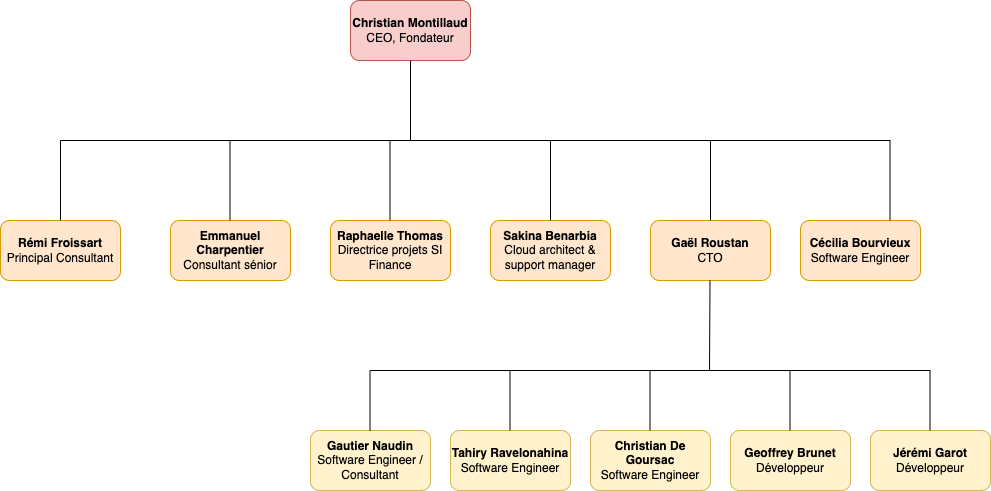
\includegraphics[scale=0.50,center]{schemas/organigramme-quartz-insight.png}
    \caption{Organigramme de Quartz-Insight}
\end{figure}
La société est gérée par monsieur Christian Montilaud.
Monsieur Gaël Roustan, est directeur technique et supervise le pôle Recherche et Développe\-ment.
Madame Cécilia Bourvieux gère un projet de test de charge pour les solutions de BI, du développement logiciel à la mise en place et l’exécution chez les clients.
Les membres du pôle R\&D ont en charge le développement des Add-Ins pour les logiciels de chez Microsoft et Google, ainsi que la création, la mise en production et la gestion des $microservices^{12}$ sous-jacents, avec l’aide de notre CTO.
Le reste des collaborateurs sont des consultants apportant leurs expertises dans leurs domaines respectifs chez nos différents clients.
\newline
\newline
Je suis donc actuellement développeur au sein du pôle R\&D, et travaille sur différents projets et $microservices^{12}$, dans le but d’améliorer ceux existants, résoudre des bugs et en créer de nouveaux lorsque cela est nécessaire.

\begin{figure}
  \section{Présentation de l'étudiant}
  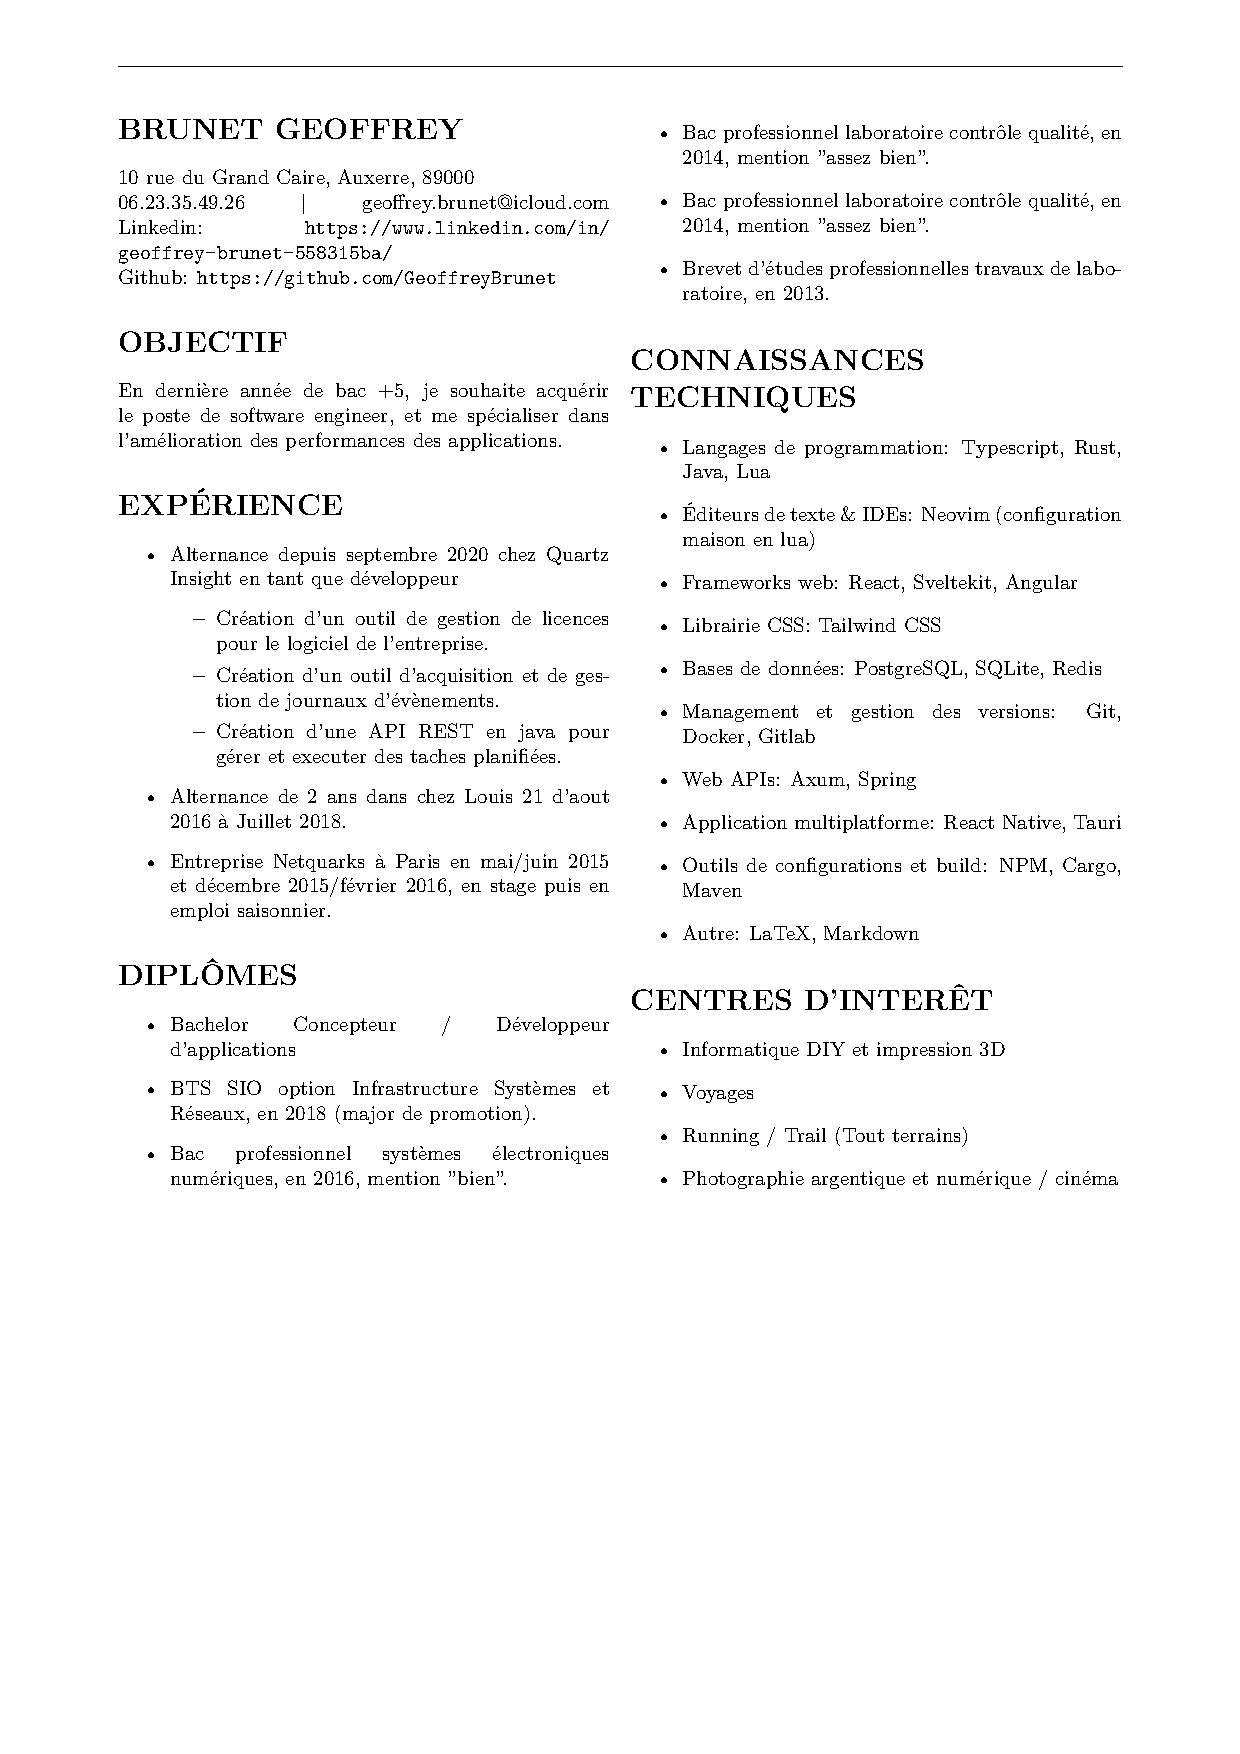
\includegraphics[scale=0.8, trim=2cm 0 0 0, clip]{CV-Geoffrey-Brunet.pdf}%
\end{figure}

\section{Activités de la structure}
Quartz-Insight est une entreprise spécialisée dans la Business Intelligence (BI) et l'Enterprise Performance Management (EPM).
Elle propose une gamme complète d'activités et de services destinés à aider les entreprises à optimiser leur gestion et à prendre des décisions éclairées. Voici un aperçu de nos principales activités:
\begin{enumerate}
  \item \textbf{Consulting en BI et EPM}: Quartz-Insight offre des services de consulting personnalisés pour accompagner les entreprises dans leur utilisation efficace des outils de BI et d'EPM tels que les serveurs Essbase, les cubes OLAP et Hyperion Planning.
    \ Les consultants de Quartz-Insight travaillent en étroite collaboration avec les clients pour comprendre leurs besoins spécifiques et proposer des solutions adaptées à leurs objectifs.
  \item \textbf{Réalisation de tests de charges sur des infrastructures de BI et d’EPM}: nous proposons une prestation de tests de charges pour les infrastructures BI et EPM des entreprises, avec divers scénarios possibles, pour tester les limites du matériel physique comme du logiciel.
    \ Le produit final est un fichier PDF contenant les résultats sous forme de graphs, ainsi qu’une proposition d’actions à mettre en place pour améliorer la résilience de l’infrastructure.
  \item \textbf{Développement de Qibates}: développement d’un logiciel en mode SAAS (Software As A Service) pour explorer diverses sources de bases de données multidimensionnelles.
    \ Un abonnement par licence par utilisateur est proposé à la vente, pour une utilisation sur Microsoft Excel ou Google Sheets, avec des accès à des sources de données diverse grâce à des connecteurs développés par nos soins. 
  \item \textbf{Conseil sur la transition RSE des entreprises}: après une implementation d’actions RSE (Responsabilité sociétale des entreprises) et de formations pour notre entreprise, nous avons décidé de proposer à nos clients une formation comprenant tous les principaux axes des actions mises en place.
    \ Nos proposons aussi une animation pour la fresque du climat, pour démontrer l’implication écologique pour les personnes comme pour les entreprises.
\end{enumerate}

\section{Présentation des activités confiées}
Voici une liste contenant les tâches qui m’ont été confiées durant mon alternance chez Quartz-Insight:
\begin{itemize}
  \item Écriture de fichiers « Dockerfile » pour la conteneurisation de nos microservices
  \item Résolution de tickets d’incidents sur l’add-in QiBates pour Google Sheets
  \item Écriture d’un logiciel de récupération de journaux d’évènements, avec une page web pour les consulter
  \item Collaboration pour développer une API REST sur un projet pour un de nos client (BNP)
  \item Transformation d’un ancien service monolithique en microservices pour la gestion des licences utilisateurs
\end{itemize}

\section{Présentation du Système d’Information}
Comme vu précédemment, le pôle Recherche et Développement édite des logiciels sous forme d’Add-In pour Google Sheets, Google Slides et Microsoft Excel, pour la manipulation de bases de données multidimensionnelles et d’outils de Planning.
Pour un soucis de performance, le traitement des données n’est pas fait sur le frontend de nos Add-Ins mais par des microservices hébergés sur nos machines virtuelles, dans un format de conteneur Docker.
\newline
\newline
Tous les microservices nécessitant d’être déployé sur des serveurs le seront sur des machines virtuelles hébergées chez notre partenaire OBS (pour Orange Business Services, filiale cloud du groupe Orange).
Ces machines virtuelles utilisent Docker pour gérer les cycles de vie des conteneurs.
Il en vas de même pour les bases de données, que nous utilisons en version managée, donc dont toute la partie serveur est gérée par OBS directement.

\chapter{Valorisation des compétences}

\section {Présentation du projet principal}
\textbf{Bloc de compétences}: A1, A4, A5
\newline
\textbf{Activité}: Réécriture et adaptation d’un monolithe en microservices et ajout de fonctionnalités face aux nouvelles contraintes
\newline
\textbf{Compétences choisies}: \begin{itemize}
  \item \textbf{A1C4} – Cartographier un système d’information existant selon les 4 niveaux (métier, fonctionnel, applicatif et infrastructure) afin d’avoir une bonne connaissance de l’ensemble de ses composants 
  \item \textbf{A1C5} – Identifier les informations sensibles, les risques, les zones critiques et les chemins d’attaque possibles d’un système d’information existant à l’aide de la cartographie afin d’aider le/la RSSI à définir une politique de sécurité
  \item \textbf{A4C6} – Définir les données de référence de l’entreprise à partir des données utilisées pour créer un référentiel de données afin d’assurer la mise à disposition de données cohérentes aux directions métiers
  \item \textbf{A5C1} – Collecter les besoins métiers des utilisateurs en menant des interviews auprès d’eux pour comprendre leurs activités et leurs contraintes métier afin d’étudier les opportunités et la faisabilité technologique d’une solution applicative spécifique ou métier
  \item \textbf{A5C2} – Concevoir une architecture applicative selon la complexité du système d’information existant de type architecture distribuée, ou micro service évolutive et tolérante aux pannes
  \item \textbf{A5C3} Développer une application adéquate selon la stratégie applicative de l’environnement en utilisant un langage de programmation approprié dans le respect du cahier des charges établi afin de répondre aux besoins utilisateurs/directions métiers
  \item \textbf{A5C5} – Effectuer les tests de la solution applicative paramétrée ou développée pour identifier les erreurs et dysfonctionnements et établir les plans de correction/d’amélioration avant sa mise en production
  \item \textbf{A5C6} –Appliquer l’intégration continue dans le cadre du développement d’une application en utilisant un outil d’intégration continue afin de vérifier la conformité de la solution et les besoins utilisateurs
  \item \textbf{A5C7} – Vérifier la conformité entre la solution développée ou paramétrée et les fonctionnalités attendues à partir des retours des directions métiers afin de rédiger la documentation et les référentiels orientés utilisateurs
  \item \textbf{A5C8} - Conduire le changement auprès des métiers lors du déploiement d’une solution applicative ou intégrée en mettant en place une démarche de participation, de communication et de formation pour accompagner les utilisateurs à l’intégration du nouvel outil dans leurs habitudes de travail
\end{itemize}

\subsection{Quelle est la finalité de cette compétence dans l’entreprise et/ou le service ?}
\subsection{En quoi consiste la compétence ?}
\subsection{Quel est le contexte de réalisation ?}
\subsection{Cette compétence a-t-elle été traversée par des évolutions majeures ces 10 dernières années ?}
\subsection{Éléments acquis par la mise en œuvre de la compétence (tant sur le plan professionnel qu’humain}

\chapter{Conclusion}

\section{Résumé}
Ce projet m'a permis d'acquérir une expérience précieuse dans le dévelop\-pement de microservices, en utilisant une combinaison de technologies telles que PostgreSQL, Spring Boot et Angular.
La réalisation de ce projet m'a permis de mettre en pratique mes connaissances théoriques acquises au cours de mes études.
J'ai dû faire face à des défis techniques, tels que la modélisation de la base de données et la mise en œuvre des fonctionnalités clés de l'application.
Ce projet m'a également sensibilisé à l'importance de la planification, de la gestion du temps et de la communication efficace dans un contexte professionnel.
J'ai appris à hiérarchiser les tâches, à gérer les priorités et à respecter les délais, tout en maintenant une communication régulière avec mon équipe et en fournissant des mises à jour régulières sur l'avancement du projet.
\newline
\newline
En conclusion, ce projet de gestion des licences utilisateurs chez Quartz-Insight a été une expérience enrichissante qui m'a permis de consolider mes compétences en développement de microservices et en gestion de projet de bout-en-bout pour un logiciel.
Je suis fier d'avoir réussi à réaliser un produit fonctionnel et utile pour les entreprises, tout en respectant les exigences et les contraintes du projet.
Je suis reconnaissant envers l'équipe de Quartz-Insight pour leur soutien et leur expertise tout au long du projet.
\section{Ouverture sur l'avenir}

\subsection{L'entreprise et ses perspectives}
Grâce à son expertise approfondie dans le domaine de la BI et de l'EPM, l’entreprise se distingue par sa capacité à proposer des stratégies de gestion efficaces, des modélisations de données précises et des analyses approfondies pour aider les entreprises à prendre des décisions éclairées.
Son équipe de consultants hautement qualifiés travaille en étroite collaboration avec les clients pour comprendre leurs besoins spécifiques et résoudre leurs problèmes, voir être pro-actifs par rapport à ceux-ci.
\newline
\newline
Les perspectives de Quartz-Insight en tant que PME sont prometteuses.
Avec son approche personnalisée, son agilité et son engagement continu envers l'innovation, l'entreprise est bien positionnée pour étendre sa clientèle et se démarquer sur le marché de la BI et de l'EPM.
La taille réduite de l'entreprise lui permet également de maintenir une culture d'entreprise forte et un haut niveau de service client, ce qui contribue à sa réputation positive.

\subsection{Le service et ses évolutions}
Grâce à la vente de licences en constante augmentation, auprès d’une clientèle de plus en plus variée, la pérennité du service est assurée. Mais de nouvelles contraintes et nouvelles améliorations peuvent être mises en place:
\begin{enumerate}
  \item \textbf{Ajout de nouveaux connecteurs et intégration de nouvelles sources de données}:
    \ En permettant l'intégration de nouvelles sources de données, telles que des bases de données supplémentaires, des services cloud ou des API externes, les utilisateurs auront une plus grande flexibilité dans l'exploration de diverses sources.
  \item \textbf{Amélioration de la supervision}:
    \ En intégrant des fonctionnalités de supervision avancées, telles que des tableaux de bord de surveillance en temps réel, des alertes automatisées en cas d'anomalies ou de dépassement de seuils, et des rapports de performance détaillés, les administrateurs et responsables pourront superviser efficacement les performances et l'utilisation de Qibates.
    \ Cela facilitera la détection précoce des problèmes, l'optimisation des ressources et la prise de décisions basées sur des données précises.
  \item \textbf{Élaboration d'un Plan de Reprise d'Activité (PRA)}:
    \ Pour assurer la continuité des opérations en cas d'incident majeur ou de catastrophe, il est essentiel de développer un PRA solide pour Qibates.
    \ Ce plan devrait inclure des procédures détaillées pour la sauvegarde régulière des données, la restauration du système, la reprise des opérations critiques, la communication avec les parties prenantes, ainsi que des tests réguliers pour s'assurer de l'efficacité du plan.
    \ Un PRA bien élaboré garantira une reprise rapide et efficace des activités en cas d'urgence, minimisant ainsi l'impact sur les utilisateurs et l'entreprise dans son ensemble.
  \item \textbf{Amélioration de la documentation}:
    \ En fournissant une documentation détaillée et des ressources de support, la prise en main de Qibates par les utilisateurs seras facilitée.
\end{enumerate}

\subsection{Les apports professionnels et personnels}
Ce projet réalisé au sein de Quartz-Insight lors de mon alternance a été une expérience professionnelle et personnelle enrichissante.
Sur le plan professionnel, j'ai pu mettre en pratique mes compétences techniques en développement de microservices, en utilisant des technologies telles que PostgreSQL, Spring Boot et Angular.
J'ai renforcé ma compréhension des processus de développement logiciel et des bonnes pratiques. 
Travailler en équipe m'a permis d'améliorer ma communication et ma collaboration.
Sur le plan personnel, j'ai gagné en confiance en moi grâce aux succès obtenus et j'ai développé mon autonomie en prenant des initiatives et en résolvant des problèmes de manière indépendante.
En résumé, ce projet m'a apporté des compétences techniques solides, renforcé ma confiance en moi, développé mon autonomie et élargi mon réseau professionnel, ce qui constituera des atouts précieux pour ma future carrière en tant qu'ingénieur logiciel.

\subsection{Avenir professionnel}
Pour mon avenir professionnel, je suis passionné par l'optimisation des performances en tant qu'ingénieur en logiciel. Je suis attiré par le développ\-ement frontend avec Svelte et TypeScript, ainsi que le développement backend avec Rust. Mon objectif est de créer des applications web rapides et performantes en réduisant les temps de réponse et en optimisant les requêtes.
J'explore également l'utilisation de Rust compilé en WebAssembly pour exécuter du code hautement performant dans les navigateurs web. Cela me permet de développer des applications web puissantes et réactives, offrant une expérience utilisateur améliorée.
En résumé, mon ambition est de contribuer à des projets stimulants axés sur l'amélioration des performances. Je souhaite devenir un ingénieur en logiciel polyvalent, capable de créer des solutions performantes en utilisant Svelte, TypeScript, Rust et WebAssembly, afin de garantir des expériences utilisateur exceptionnelles et d'optimiser l'efficacité des systèmes.

\end{document}
